%%%%%%%%%%%%%%%%%%%%%%%%%%%%%%%%%%%%%%%%%%%%%%%%%%%%%%%%%%%%%%%%%%%%%%
% Original Source: Dave Richeson (divisbyzero.com), Dickinson College
% Modified By: Chen Yiyang
% 
% A one-size-fits-all LaTeX cheat sheet. Kept to two pages, so it 
% can be printed (double-sided) on one piece of paper
% 
% Feel free to distribute this example, but please keep the referral
% to divisbyzero.com
% 
% Guidance on the use of the Overleaf logos can be found here:
% https://www.overleaf.com/for/partners/logos 
%%%%%%%%%%%%%%%%%%%%%%%%%%%%%%%%%%%%%%%%%%%%%%%%%%%%%%%%%%%%%%%%%%%%%%

\documentclass[10pt,landscape,letterpaper]{article}
\usepackage{amssymb}
\usepackage{amsmath}
\usepackage{amsthm}
\usepackage{physics} % for vectors
%\usepackage{fonts}
\usepackage{multicol,multirow}
\usepackage{spverbatim}
\usepackage{graphicx}
\usepackage{ifthen}
\usepackage[landscape]{geometry}
\usepackage{listings} % for code block
\usepackage[colorlinks=true,urlcolor=olgreen]{hyperref}
\usepackage{booktabs}
\usepackage{fontspec}
\setmainfont[Ligatures=TeX]{TeX Gyre Pagella}
\setsansfont{Fira Sans}
\setmonofont{Inconsolata}
\usepackage{unicode-math}
\setmathfont{TeX Gyre Pagella Math}
\usepackage{microtype}

\usepackage{empheq}

% new:
\def\MT@is@uni@comp#1\iffontchar#2\else#3\fi\relax{%
  \ifx\\#2\\\else\edef\MT@char{\iffontchar#2\fi}\fi
}
\makeatother

\ifthenelse{\lengthtest { \paperwidth = 11in}}
    { \geometry{margin=0.4in} }
	{\ifthenelse{ \lengthtest{ \paperwidth = 297mm}}
		{\geometry{top=1cm,left=1cm,right=1cm,bottom=1cm} }
		{\geometry{top=1cm,left=1cm,right=1cm,bottom=1cm} }
	}
\pagestyle{empty}
\makeatletter
\renewcommand{\section}{\@startsection{section}{1}{0mm}%
                                {-1ex plus -.5ex minus -.2ex}%
                                {0.5ex plus .2ex}%x
                                {\sffamily\large}}
\renewcommand{\subsection}{\@startsection{subsection}{2}{0mm}%
                                {-1explus -.5ex minus -.2ex}%
                                {0.5ex plus .2ex}%
                                {\sffamily\normalsize\itshape}}
\renewcommand{\subsubsection}{\@startsection{subsubsection}{3}{0mm}%
                                {-1ex plus -.5ex minus -.2ex}%
                                {1ex plus .2ex}%
                                {\normalfont\small\itshape}}
\makeatother
\setcounter{secnumdepth}{0}
\setlength{\parindent}{0pt}
\setlength{\parskip}{0pt plus 0.5ex}
% -----------------------------------------------------------------------

\usepackage{academicons}

\begin{document}

\definecolor{mathBlue}{cmyk}{1,.72,0,.38}
\definecolor{defOrange}{cmyk}{0, 0.5, 1, 0.3}
\definecolor{codeInlineRed}{cmyk}{0, 0.9, 0.9, 0.45}
\definecolor{light-gray}{gray}{0.95}

\everymath{\color{mathBlue}}
\everydisplay{\color{mathBlue}}

% for vector notation in this module
\newcommand{\vect}[1]{\boldsymbol{#1}}
\newcommand{\deff}[1]{\textcolor{defOrange}{\textbf{#1}}}
\newcommand{\codein}[1]{\textcolor{codeInlineRed}{\texttt{#1}}}
\newcommand{\citeqn}[1]{\underline{\textit{#1}}}

\lstset{frame=tb,
  language=C++,
  backgroundcolor=\color{light-gray},
  basicstyle={\footnotesize\ttfamily},
  tabsize=3
}

\footnotesize
%\raggedright

\begin{center}
  {\huge\sffamily\bfseries CS3241 Cheatsheet} \huge\bfseries\\
  by Yiyang, AY22/23
\end{center}
\setlength{\premulticols}{0pt}
\setlength{\postmulticols}{0pt}
\setlength{\multicolsep}{1pt}
\setlength{\columnsep}{1.8em}
\begin{multicols}{3}


% -----------------------------------------------------------------------
\section{Overview}
\subsection{Graphics Basics}
\deff{Addictive Colour} - Form a colour by adding amounts of three primaries (RGB).\\
\deff{Subtractive Colour} - Form Form a colour by filtering white with Cyan (C), Magenta (M), and Yellow (Y). \underline{Note}: For subtractive colours, M absorbs G and allows R \& B to pass through.


\subsection{OpenGL Basics}
Polygons in OpenGL need to be \textbf{Simple} (edges cannot cross), \textbf{Convex}, and \textbf{Flat} (all vertices in the same plane), or they will not be displayed correctly.

\smallskip

Colour info is stored in each vertex of a polygon, and the shading mode determines how the polygon is coloured: \\
\deff{Smooth \textasciitilde} - Interpolation of vertex colours across polygon. The default setting. \codein{glShadeModel(GL\_SMOOTH)}.
\\
\deff{Flat \textasciitilde} - Fill colour is colour of first vertex. \codein{glShadeModel(GL\_FLAT)}.


\smallskip

\deff{Hidden Surface Removal} - It deals with 3D objects overlapping over one another from our perspective, by using an extra \deff{z-buffer} that saves depth information.





\section{Interaction}
\subsection{Overview}
Input devices generate \deff{Triggers}, namely signals, and return \deff{Measures}, which are trigger with other meta-info from the input devices, to the OS. Each trigger generates an \deff{Event} whose measure is put in an \deff{Event Queue} to be examined by the user program.
\\
The user program defines a \deff{Callback} for each type of event to GLUT and it is executed when the event occurs.


\subsection{Positioning in Callbacks}
Window systems (such as mouse \& motion callbacks) measure positions with origin at \textbf{top-left corner}. OpenGL measures positions with origin at \textbf{bottom-left corner}. Conversion:
\[
x_\text{opengl} = x_\text{win}, \;\; y_\text{opengl} = h - 1 - y_\text{win}
\]


\subsection{Animation}
\deff{Double Buffering} - The usage of two \textbf{colour buffers} for display where the \deff{Front Buffer} displays and the \deff{Back Buffer} is written to. It minimises flickering in animation.
\\
\underline{Note}: Two identical buffers, switched once writing to back is done.





\section{Geometry}
\subsection{Representation}
\deff{Affine Space} - A frame formed by an origin point and basis vectors.

\smallskip

\deff{Homogeneous Coordinates} \textasciitilde A 4D system for 3D points \& vectors.
\begin{itemize}
    \item Vector $v = [\alpha_1, \alpha_2, \alpha_3, 0]^T = (\alpha_1, \alpha_2, \alpha_3)$
    \item Point $p = [\beta_1, \beta_2, \beta_3, w]^T = (\frac{\beta_1}{w}, \frac{\beta_2}{w}, \frac{\beta_3}{w})$
\end{itemize}
\underline{Note}: [1] All Homogeneous Coordinate elements are denoted as \textbf{Column Vectors}. [2] $\text{Point} + \text{Vector} = \text{Point}$. [3] Representation for each point is non-unique. We typically use $w=1$. \deff{Perspective Division} is the process of dividing $x, y, z$ by $w$.


\subsection{Transformation}
All transformations can be expressed as a $4 \times 4$ matrix, \textbf{pre-multiplied} to the Homogeneous Coordinates.
\\
\underline{Note}: $p' = ABp$ is to apply transformation $B$ then $A$ to element $p$.
\subsubsection{Translation}
\[
T(d_x, d_y, d_z) = 
\begin{bmatrix}
1       & 0         &  0        & d_x       \\
0       & 1         &  0        & d_y       \\
0       & 0         &  1        & d_z       \\
0       & 0         &  0        & 1
\end{bmatrix}
\]

\subsubsection{Rotation}
\begin{align*}
R_x(\theta) &= 
\begin{bmatrix}
1           & 0             &  0            & 0      \\
0           & \cos\theta    &  -\sin\theta  & 0      \\
0           & \sin\theta    &  \cos\theta   & 0      \\
0           & 0             &  0            & 1
\end{bmatrix} 
\\
R_y(\theta) &= 
\begin{bmatrix}
\cos\theta  & 0             &  \sin\theta   & 0      \\
0           & 1             &  0            & 0      \\
-\sin\theta & 0             &  \cos\theta   & 0      \\
0           & 0             &  0            & 1
\end{bmatrix} 
\\
R_z(\theta) &=
\begin{bmatrix}
\cos\theta  & -\sin\theta   & 0             & 0         \\
\sin\theta  & \cos\theta    & 0             & 0         \\
0           & 0             & 1             & 0         \\
0           & 0             & 0             & 1
\end{bmatrix}
\end{align*}

\subsubsection{Scaling}
\[
S(s_x, s_y, s_z) = 
\begin{bmatrix}
s_x     & 0         & 0         & 0     \\
0       & s_y       & 0         & 0     \\
0       & 0         & s_z       & 0     \\
0       & 0         & 0         & 1
\end{bmatrix}
= diag(s_x, s_y, s_z, 1)
\]

\subsubsection{Inverse of Transformation Matrices}
\begin{itemize}
    \item $T^{-1}(d_x, d_y, d_z) = T(-d_x, -d_y, -d_z)$
    \item $R^{-1} = R^T$, as all $R$ orthogonal
    \item $S^{-1}(s_x, s_y, s_z) = S(1/s_x, 1/s_y, 1/s_z)$
\end{itemize}

\subsubsection{Combinations of Transformation}
\textbf{General Rotation about Origin}: $R(\theta) = R_z(\theta_z)R_y(\theta_y)R_x(\theta_x)$, where $\theta_x, \theta_y, \theta_z$ are the Euler angles.
\\
\textbf{Rotation about Arbitrary Point}: $M = T(p_f) R(\theta) T(-p_f)$, where $p_f$ is the point and $\theta$ rotational angle.
\\
\underline{Note}: Matrix ordering is the reverse of the actual transformation's. 

\subsection{OpenGL Transformation}
For each matrix mode, \deff{Current Transformation Matrix} (CTM) stores the $4 \times 4$ homogeneous coordinate matrix, as part of the state and it is applied to all vertices in the pipeline. Some matrix modes include Model-View (\codein{GL\_MODEVIEW}) and Projection (\codein{GL\_PROJECTION}).
\\
OpenGL also maintains a stack for each matrix mode.





\section{Camera \& Viewing}
OpenGL Spaces: \deff{Object Space}, for modelling each object where the object is centred in the frame. \deff{World Space}, a common frame for all objects, and for defining lightning and camera pose. \deff{Camera Space}, the local frame for camera where it is at the origin and looking into the \textbf{Negative z-direction}, initially the same as the world frame.

\smallskip

An OpenGL \deff{Viewport} defines a rectangular region of the window in which OpenGL can draw.
\\
\underline{Note}: [1] A window can have multiple viewports. [2] A viewport can be larger than the window, and whatever inside the viewport but outside the window will not be displayed.


\subsection{Transformations}
\deff{View Transformation} - Transform points from World Frame to Camera Frame. The transformation matrix
\[
M_\text{view} = RT
\]
where $T$ moves camera position back to world origin, and $R$ rotates axes of camera to coincide with world frame's.
\\
View transformation for normal vectors:
\[
M_n = \big( M_t^{-1} \big)^T
\]
, where $M_t$ is the upper left $3 \times 3$ sub-matrix of $M_\text{view}$.

\smallskip

\deff{Projection Transformation} - Specify a \textbf{View / Clipping Volume} in the camera frame, and project the volume to a $2 \times 2 \times 2$ cube centred at origin, known as the \deff{Normalised Device Coordinate} (NDC) / \deff{Canonical View Volume}.
\\
\underline{Note}: It preserves depth order and lines.


\subsection{Projections}
Types of projection
\begin{itemize}
    \item \deff{Perspective projection} - Projectors converge at centre of projection. Objects further from viewer are projected smaller.
    \item \deff{Parallel Projection} - Projectors are parallel. One special case \deff{Orthographic Projection} is where projectors are orthogonal to projection surface.
\end{itemize}

Perspective Transformation for Homogeneous Coordinates
Any point $q = [x, y, z, 1]^T$ projected perspectively onto vertical plane at $z = d < 0$ will be at $(xd/z, yd/z, d)$, equivalent to $p = [x, y, z, z/d]^T = Mq$ for
\[
M = 
\begin{bmatrix}
1       & 0         &  0        & 0       \\
0       & 1         &  0        & 0       \\
0       & 0         &  1        & 0       \\
0       & 0         &  1/d      & 1
\end{bmatrix}
\]

\subsubsection{OpenGL Projection Matrix Equivalences}
\codein{glOrtho(L, R, B, T, N, F)}:
\[
M_\text{ortho} = 
\begin{bmatrix}
\frac{2}{R-L}   & 0             &  0                & -\frac{R+L}{R_L}       \\
0               & \frac{2}{T-B} &  0                & -\frac{T+B}{T-B}       \\
0               & 0             &  \frac{-2}{F-N}   & -\frac{F+N}{F-N}       \\
0               & 0             &  0                & 1     
\end{bmatrix}
\]

\codein{glFrustum(L, R, B, T, N, F)}:
\[
M_\text{persp} = 
\begin{bmatrix}
\frac{2N}{R-L}  & 0                 & \frac{R+L}{R-L}   & 0                     \\
0               & \frac{2N}{T-B}    & \frac{T+B}{T-B}   & 0                     \\
0               & 0                 & -\frac{F+L}{F-L}  & -\frac{2FN}{F-L}      \\
0               & 0                 & -1                & 0
\end{bmatrix}
\]





\section{Rendering}
\deff{Primitive Assembly} - The stage where primitive types are recalled and  their processed vertices are collected for polygons, so that we can redefine the primitive for clipping and rasterization.

\subsection{Clipping}
\subsubsection{Brute Force Approach}
Compute intersections with all sides of the clipping window.
\\
\underline{Analysis}: Inefficient, require one division per intersection.


\subsubsection{2D Cohen-Sutherland Algorithm}
Define \deff{Outcode} $b_0 b_1 b_2 b_3$ where bit is $1$ iff it is outside $y_\text{max}$, $y_\text{min}$, $x_\text{max}$, $x_\text{min}$ respectively (top, btn, right, left) for each endpoint.
\\
For a line with 2 endpoints $A$ and $B$, four cases to consider:
\begin{itemize}
    \item \codein{Out(A) == Out(B) == 0} - Both points inside all 4 boundaries. Accept the entire line.
    \item \codein{Out(A) == 0 \&\& Out(B) != 0} - One point inside all and one outside some, at least one intersection.
    \item \codein{Out(A) \& Out(B) != 0} - Both points outside the same boundary. Discard the entire line.
    \item \codein{Out(A) \& Out(B) == 0 \&\& Out(A) | Out(B) != 0} - May or may not be intersection. Most complicated.
\end{itemize}
\underline{Analysis}: [1] Efficient, as it filters out simple cases. [2] Yet, still need computation for complicated cases. [3] Can extend to 3D using $6$-digit outcodes.


\subsubsection{Polygon Clipping}
Clipping a polygon may yield multiple polygons, but clipping a \textbf{convex polygon} can yield at most one other.
\\
\deff{Tessellation} - replace concave polygons with a set of smaller simple polygons, typically triangles. Tessellation enables simpler clipping.


\subsubsection{AABB Clipping Algorithm}
\deff{Axis-Aligned Bounding Box} (AABB) - 1) Draw a bounding box for the polygon. 2) Consider whether and whereh we need to perform detailed clipping. 
\\
\underline{Analysis}: Similar idea of "easy filtering first".


\subsection{Rasterisation}
\deff{Rasterisation} - The process of determining which pixels are inside primitive specified by a set of vertices. It produces a set of fragments.
\\
\deff{Fragments} \textasciitilde “Potential pixels”, with a pixel location and attributes such as colour and depth.

\subsubsection{DDA Algorithm}
Simple iterative method that moves along one axis one pixel at a time. To draw a line $y = mx + b$ from $(x_0, y_0)$ to $(x_e, y_e)$:
\begin{lstlisting}
for (x=x0, y=y0; x <= xe; x++) {
    write_pixel(x, round(y), color);
    y += m;
}
\end{lstlisting}
\underline{Analysis}: [1] Simple, and applicable to curves as well. [2] Inefficient due to many floating point calculations. [3] Lines rasterised are discontinuous when $|m| > 1$. Solution is to flip roles of $x$ and $y$.


\subsubsection{Bresenham’s Algorithm}
Use a \deff{Decision Variable}, $p_k$ to determine which $y$-value to rasterise for every $x$.

\begin{enumerate}
    \item Input line and store left end in $(x_0, y_0)$. Assume $|m| <= 1$.
    \item Calculate constants $\triangle x, \triangle y, 2\triangle y, 2\triangle y - 2\triangle x$.
    \item Fill $(x_0, y_0)$, and obtain $ p_0 = 2\triangle y - \triangle x $.
    \item At each $x_k$ along the line, starting at $k=0$, perform the following test: [1] If $p_k < 0$, then next point is $(x_k + 1, y_k)$, and $p_{k+1} = p_k + 2\triangle y$. [2] Otherwise, next point $(x_k+1, y_k+1)$ and $p_{k+1} = p_k + 2\triangle y - 2 \triangle x$.
    \item Repeat Step 4 for $\triangle x - 1$ more times.
\end{enumerate}

\underline{Analysis}: [1] Only applicable to line (and circle) rasterisation. [2] Efficient, due to no floating points. 


\subsubsection{Polygon Rasterisation Algorithms}
\deff{Scan-Line Fill Algorithm} - [1] First tessellate if concave. [2] Compute colours \& depths for vertices. [3] For each horizontal line, interpolate colours and z-values.

\deff{Floor Fill Algorithm} - Start with one point inside the polygon, expand to 4 directions using BFS recursively.


\subsection{Hidden Surface Removal}
\deff{Painter's Algorithm} - Render polygons in back-to-front order so that polygons behind others are simply painted over.
\\
\underline{Analysis}: It involves \deff{Depth Sorting}, with time complexity $O(n \log n)$ for $n$ polygons.

\smallskip

\deff{Back-Face Culling} - Eliminate polygon if it is \textbf{back-facing} and invisible, i.e. when $N_p \cdot N < 0$.
\\
\underline{Note}: Need to specify polygon vertices in Anti-Clockwise order to ensure correct orientation for convex polygons.

\smallskip

\deff{Image-Space Approaches} - Look at each pixel / projector and find closest of all polygons along that pixel. 
\\
\underline{Example}: Ray Tracing, z-Buffering (using a z-buffer / depth buffer).
\\
\underline{Analysis}: Complexity $O(nmk)$ for $k$ polygons and frame buffer sized $n \times m$.






% \noindent\rule{8cm}{0.4pt}




\section{Others}
% % For intermediate results, code usage, and images/screenshots
% \subsection{From Tutorials \& Assignments}
% \subsection{From Past Year Papers}
\subsection{Diagrams}
Colour Theory, Transformation Pipeline
\\
\begin{center}
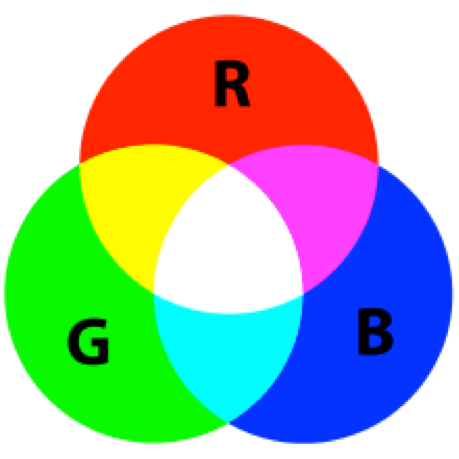
\includegraphics[width=4cm]{img/01_colours.png}
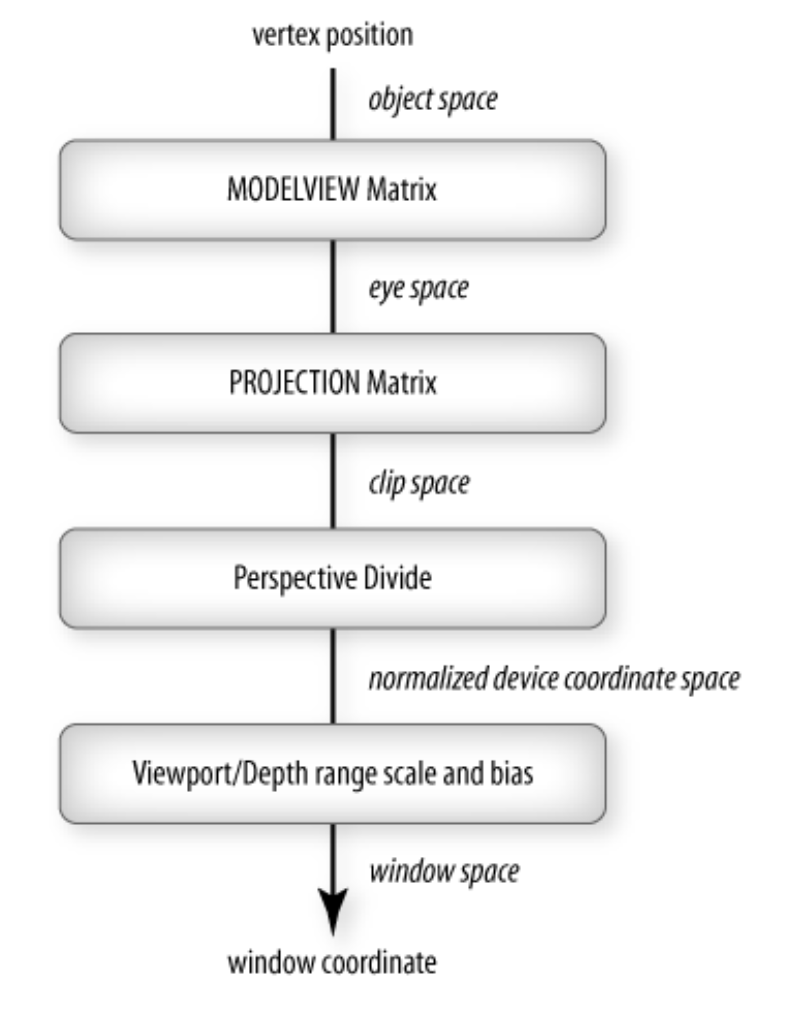
\includegraphics[width=4cm]{img/03_transformation_pipeline.png}
\end{center}

Rendering Pipeline
\\
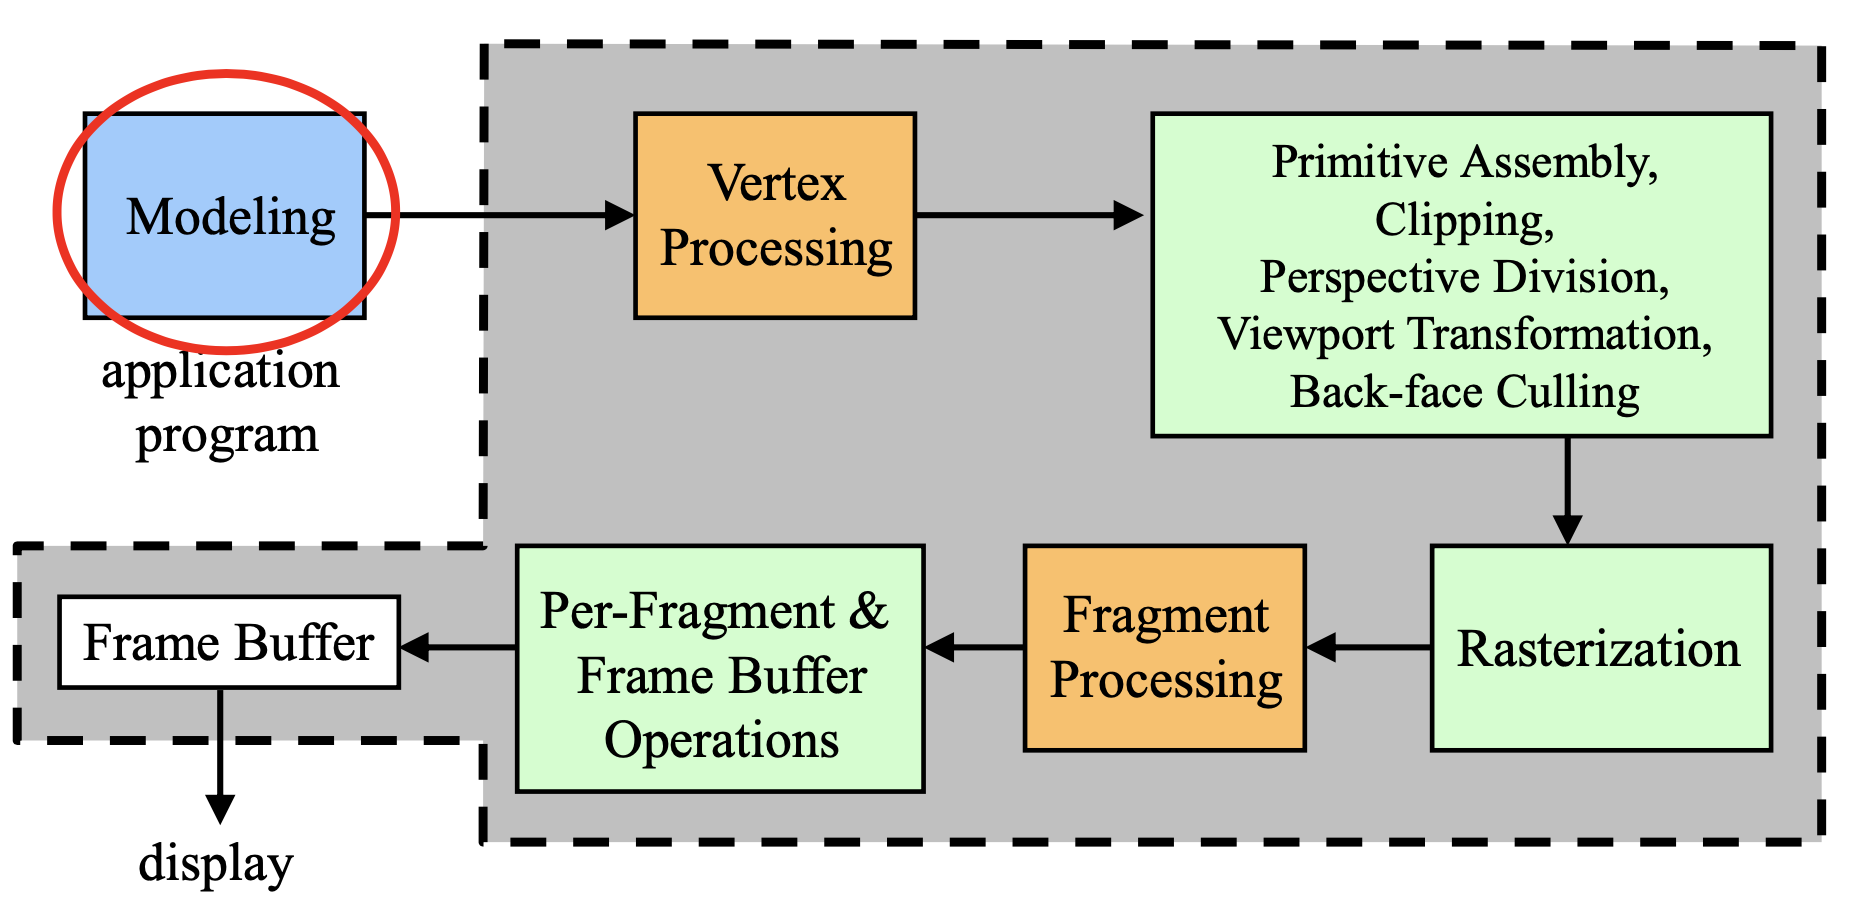
\includegraphics[width=8cm]{img/02_rendering_pipeline.png}

gluLookAt Coordinate Specification
\\
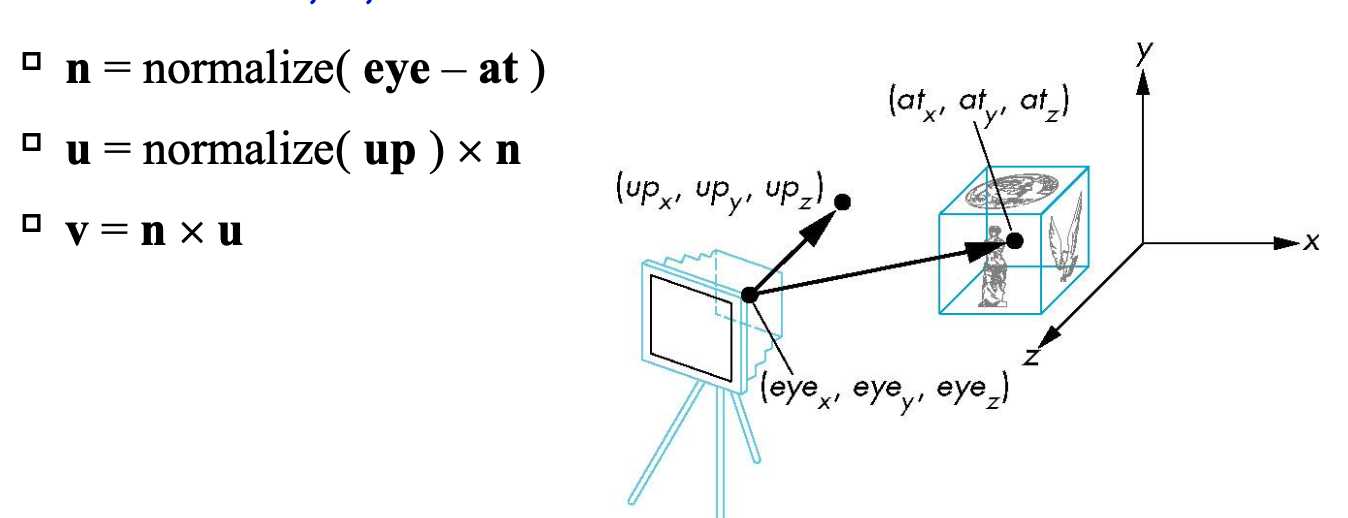
\includegraphics[width=8cm]{img/04_glulookat.png}



% % 5, transformation pipeline
% %5  up vectors
% %6, Rendering pipeline


\noindent\rule{8cm}{0.4pt}




\section{OpenGL Reference}
\subsection{Miscellaneous}
\subsubsection{Settings}
\codein{glutInitDisplayMode(...|GLUT\_DOUBLE)} uses Double Buffering, as compared to \codein{GLUT\_SINGLE} for Single Buffering.

\smallskip

\codein{glViewport(u, v, w, h)} - Define the rectangular viewport.



\subsection{Callback-Related}
\codein{glutDisplayFunc(void (*func)(void))} - when GLUT determines the window to be refreshed (e.g. opened, reshaped, exposed etc.)
\\
\codein{glutIdleFunc} - when there is no trigger (e.g. for animation).
\\
\codein{glutMotionFunc} - when mouse on hold and moving.
\\
\codein{glutPassiveMotionFunc} - when mouse moving but not on hold.
\\
\codein{glutTimerFunc(unsigned int msecs, void (*func)(int value), value)} - Set a timer and trigger the callback when timer elapses.
\\
Other common trigger callbacks: \codein{glutMouseFunc}, \codein{glutReshapeFunc}, \codein{glutKeyboardFunc}.

\smallskip

\codein{glutPostRedisplay()} - Set a flag for posting redisplay, which avoids frequent repeated execution.


\subsection{OpenGL Matrices \& Transformation}
\codein{glMatrixMode(GLenum mode)} - Specify the current matrix mode. Modes are \codein{GL\_MODELVIEW}, \codein{GL\_PROJECTION}, \codein{GL\_TEXTURE} or \codein{GL\_COLOR}.

\smallskip

\subsubsection{Transformations}
\codein{glLoadIdentity()} - Override CTM with $I_{4}$.
\\
\codein{glTranslatef(dx, dy, dz)} - Post-mul. translation matrix to CTM.
\\
\codein{glRotatef(theta, vx, vy, yz)} - Post-mul. rotation matrix to CTM.
\\
\codein{glScalef(sx, sy, sz)} - Post-mul. scaling matrix to CTM.
\\
\codein{glLoadMatrixf(m)} - Override CTM with matrix $m_{4 \times 4}$.
\\
\codein{glMultMatrixf(m)} - Post-mul. $m_{4 \times 4}$ to CTM.
\\
\underline{Note}: [1] Each has a Double(\codein{gl...d}) and a Float (\codein{gl...f}) format. [2] $m$ is a 1D array of length 16, ordered by column.

\subsubsection{Matrix Stacks}
\codein{glPushMatrix()} - Push CTM to the stack, and duplicate the CTM.
\\
\codein{glPopMatrix()} - Pop top matrix from the stack and replace CTM.
\\
\underline{Note}: Typically an indentation is applied for every Push-Pop pair.


\subsection{Camera \& Viewing}
\codein{gluLookAt(eyex, eyey,eyez, atx, aty, atz, upx, upy, upz)} \\ - Create a view transformation matrix for the camera specified. \codein{eye*} specify the camera location, \codein{at*} specify where to look at, and \codein{up*} is \deff{Up-Vector} for orientation of camera.
\\
\underline{Note}: [1] The up vector does not need to be perpendicular to Eye-At. [2] The up is usually $(0, 1, 0)$.

\smallskip

\codein{glOrtho(left, right, bottom, top, near, far)} - Post-mul. to CTM the orthographic projection matrix.
\\
\underline{Note}: It will map $(-\text{near}, -\text{far})$ to $(-1, 1)$.

\codein{glFrustum(left, right, bottom, top, near, far)} - Post-mul. to CTM the perspective projection matrix.
\\
\underline{Note}: [1] LRBT all refer to the locations on the near plane. [2] It will map $(-\text{near}, -\text{far})$ to $(-1, 1)$.

\codein{gluPerspective(fovy, aspect, near, far)} - Post-mul. to CTM the "central \& symmetric" perspective projection matrix.
\\
\underline{Note}: \codein{fovy} vertical field of view angle in degrees. \codein{aspect} $w / h$ ratio.


% 5. M_persp equiv matrix for glFrustum



\end{multicols}
\end{document}
